\documentclass[11pt,a4paper]{article}
\usepackage[utf8]{inputenc}
\usepackage[T1]{fontenc}
\usepackage[brazil]{babel}
\usepackage{lmodern}
\usepackage{amsmath,amssymb,amsthm}
\usepackage{graphicx}
\usepackage{booktabs}
\usepackage{array}
\usepackage[margin=2.5cm]{geometry}
\usepackage{listings}
\usepackage{xcolor}
\usepackage[hidelinks]{hyperref}
\usepackage{caption}
\usepackage{float}

\lstset{language=Python, basicstyle=\ttfamily\small, keywordstyle=\color{blue!60!black},
  commentstyle=\color{green!40!black}, stringstyle=\color{red!50!black},
  frame=single, framerule=0.3pt, breaklines=true, columns=fullflexible,
  literate={á}{{\'a}}1 {é}{{\'e}}1 {í}{{\'i}}1 {ó}{{\'o}}1 {ú}{{\'u}}1 {ã}{{\~a}}1
           {õ}{{\~o}}1 {ç}{{\c c}}1 {ê}{{\^e}}1 {â}{{\^a}}1 {ô}{{\^o}}1 {à}{{\`a}}1
           {ε}{{$\varepsilon$}}1 {²}{{$^2$}}1 {·}{{$\cdot$}}1}

\newtheorem{proposicao}{Proposição}
\newcommand{\fl}{\operatorname{fl}}
\renewcommand{\Im}{\operatorname{Im}}
\renewcommand{\Re}{\operatorname{Re}}

\title{Diferenciação automática, passo complexo e diferenças finitas:\\
\large por que só os dois primeiros atingem o arredondamento unitário\\[4pt] \normalsize Parte teórica}
\author{Felipe M. Figueira \and Lucas Cavalhiosa}
\date{\small Seminário --- outubro de 2026}

\begin{document}
\maketitle

\begin{abstract}
Diferenças finitas aproximam derivadas por quocientes de diferenças e, em aritmética de ponto flutuante, estão sujeitas a um compromisso inevitável entre erro de truncamento e erro de cancelamento: o melhor erro alcançável com um método de ordem $p$ é da ordem de $u^{p/(p+1)}$, onde $u\approx1{,}1\times10^{-16}$ é o arredondamento unitário. Mostramos que o passo complexo elimina a subtração (e com ela o termo $u/h$), e que a diferenciação automática no modo direto, formalizada por números duais, elimina também o truncamento. Ambos atingem erro da ordem de $u$. O preço é pago em generalidade: o passo complexo exige funções analíticas implementadas com operações ``seguras'' para complexos; os duais exigem que todo o programa seja escrito em operações sobrecarregáveis. Esta versão reúne apenas a parte teórica do trabalho (deduções A1--A3); a implementação e os experimentos estão no relatório completo.
\end{abstract}

\tableofcontents

%======================================================================
\section{Introdução}

Derivadas aparecem em toda parte em computação científica: métodos de Newton, otimização, análise de sensibilidade, treinamento de redes neurais. Há quatro formas de obtê-las num computador: (i) derivação manual, (ii) derivação simbólica, (iii) aproximação numérica por diferenças finitas e (iv) diferenciação automática (AD). Este trabalho compara (iii) e (iv), com uma técnica intermediária, o \emph{passo complexo}~\cite{squire1998,martins2003}, que serve de ponte conceitual entre as duas.

A pergunta central é:

\begin{quote}
\emph{Por que diferenças finitas nunca atingem erro $u$, e o que exatamente o passo complexo e a AD fazem para atingi-lo? Qual é o custo em generalidade (tipos de $f$ aceitos) e em implementação?}
\end{quote}

\paragraph{Modelo de ponto flutuante.} Usamos o modelo padrão: para $a,b$ números de máquina e $\circ\in\{+,-,\times,/\}$,
\begin{equation}
\fl(a\circ b) = (a\circ b)(1+\delta), \qquad |\delta|\le u = 2^{-53}\approx 1{,}11\times 10^{-16}
\end{equation}
em precisão dupla. Supomos também que a avaliação de $f$ é feita com erro relativo da ordem de $u$: $\hat f(x) = f(x)(1+\delta_f)$, $|\delta_f|\lesssim u$.\footnote{Na prática $|\delta_f|$ pode ser alguns múltiplos de $u$; isso muda constantes, não expoentes.}

Esta versão contém apenas a parte teórica (Seções~\ref{sec:fd} a~\ref{sec:segunda}). A implementação da classe \texttt{Dual}, os testes e os experimentos estão no relatório completo e no notebook \texttt{experimentos\_ad.ipynb}, que também gera a figura da Seção~\ref{sec:segunda}.

%======================================================================
\section{Diferenças finitas: o compromisso truncamento $\times$ cancelamento}
\label{sec:fd}

\subsection{Diferença progressiva}
Por Taylor, $f(x+h) = f(x) + hf'(x) + \tfrac{h^2}{2}f''(\xi)$, logo
\begin{equation}
D_+(h) = \frac{f(x+h)-f(x)}{h} = f'(x) + \underbrace{\tfrac{h}{2}f''(\xi)}_{\text{truncamento}} .
\end{equation}
Em ponto flutuante, cada avaliação tem erro absoluto até $u|f|$. Como $f(x+h)\approx f(x)$, a subtração é exata (lema de Sterbenz) mas \emph{revela} esses erros: a diferença calculada tem erro absoluto de até $2u|f|$, que é dividido por $h$:
\begin{equation}
|\hat D_+(h) - f'(x)| \lesssim \frac{h}{2}|f''| + \frac{2u|f|}{h} .
\label{eq:erro-prog}
\end{equation}
Esse é o \textbf{cancelamento catastrófico}: os primeiros dígitos de $f(x+h)$ e $f(x)$ coincidem e se anulam, sobrando apenas os dígitos contaminados por arredondamento. Minimizando~\eqref{eq:erro-prog} em $h$:
\begin{equation}
h^\ast = 2\sqrt{\frac{u|f|}{|f''|}}, \qquad E(h^\ast) = 2\sqrt{u|f||f''|} = O(u^{1/2}).
\end{equation}

\subsection{Diferença centrada}
Subtraindo as expansões de $f(x\pm h)$, os termos pares se cancelam:
\begin{equation}
D_c(h) = \frac{f(x+h)-f(x-h)}{2h} = f'(x) + \frac{h^2}{6}f'''(x) + \frac{h^4}{120}f^{(5)}(x) + O(h^6).
\label{eq:centrada}
\end{equation}
O numerador tem erro de até $2u|f|$, dividido por $2h$, e portanto
\begin{equation}
E_c(h) \approx \frac{h^2}{6}|f'''| + \frac{u|f|}{h}, \qquad
h^\ast = \left(\frac{3u|f|}{|f'''|}\right)^{1/3}, \qquad E_c(h^\ast) = O(u^{2/3}).
\end{equation}

\subsection{Extrapolação de Richardson}
Combinando $D_c(h)$ e $D_c(h/2)$ para eliminar o termo $h^2$ de~\eqref{eq:centrada},
\begin{equation}
D_R(h) = \frac{4D_c(h/2)-D_c(h)}{3} = f'(x) - \frac{h^4}{480}f^{(5)}(x) + O(h^6).
\end{equation}
Os coeficientes amplificam o arredondamento: $\frac43\cdot\frac{2u|f|}{h} + \frac13\cdot\frac{2u|f|}{2h} = \frac{3u|f|}{h}$. Assim
\begin{equation}
E_R(h)\approx \frac{h^4}{480}|f^{(5)}| + \frac{3u|f|}{h}, \qquad h^\ast = \left(\frac{360\,u|f|}{|f^{(5)}|}\right)^{1/5},\qquad E_R(h^\ast)=O(u^{4/5}).
\end{equation}

\subsection{O resultado geral}
\begin{proposicao}
Seja $D_p(h)$ uma fórmula de diferenças finitas de ordem $p$ para $f'(x)$, isto é, uma combinação $\frac1h\sum_k c_k f(x+kh)$ com $\sum_k c_k=0$ e erro de truncamento $C_ph^p$. Então o erro total satisfaz $E(h)\approx C_ph^p + K_pu|f|/h$, cujo mínimo é
\[
E(h^\ast) \asymp u^{p/(p+1)} \quad\text{com}\quad h^\ast\asymp u^{1/(p+1)}.
\]
Como $p/(p+1)<1$ para todo $p$ finito, nenhuma fórmula de diferenças finitas atinge erro $O(u)$.
\end{proposicao}

A condição $\sum_kc_k=0$ é exatamente o que torna a fórmula exata para constantes --- e é ela que obriga a subtrair valores próximos de $f$. \emph{O termo $u/h$ é consequência inevitável da subtração.} Aumentar a ordem empurra o expoente para perto de 1, mas as constantes $K_p$ crescem e o expoente nunca chega lá. Além disso, para $h<u|x|$ tem-se $\fl(x+h)=x$ e a fórmula devolve exatamente zero.

%======================================================================
\section{O passo complexo (A1)}
\label{sec:cs}

Se $f$ é real em eixo real e analítica numa vizinhança de $x$, podemos expandir em $x+ih$:
\begin{equation}
f(x+ih) = f(x) + ihf'(x) - \frac{h^2}{2}f''(x) - i\frac{h^3}{6}f'''(x) + \frac{h^4}{24}f^{(4)}(x) + \cdots
\label{eq:taylor-complexo}
\end{equation}
Como $f(x), f'(x),\dots$ são reais, separamos partes real e imaginária:
\begin{align}
\Im f(x+ih) &= hf'(x) - \frac{h^3}{6}f'''(x) + O(h^5), \\
\Re f(x+ih) &= f(x) - \frac{h^2}{2}f''(x) + O(h^4). \label{eq:parte-real}
\end{align}
Logo
\begin{equation}
\boxed{\;f'(x) = \frac{\Im f(x+ih)}{h} + \frac{h^2}{6}f'''(x) + O(h^4).\;}
\end{equation}

\paragraph{Truncamento.} O erro é $O(h^2)$, com o mesmo módulo $h^2|f'''|/6$ da diferença centrada e sinal oposto (verificado numericamente no notebook: para $h=10^{-3}$ ambos dão $9{,}472\times10^{-6}$ com sinais trocados).

\paragraph{Por que não há termo $u/h$.} Na centrada, o numerador é $f(x+h)-f(x-h)$, a diferença de dois números de tamanho $|f|$ cujo resultado tem tamanho $2h|f'|$: o erro absoluto $u|f|$ de cada parcela vira erro \emph{relativo} $u|f|/(h|f'|)$ no resultado. No passo complexo não há subtração alguma: a quantidade de interesse, $hf'(x)$, \emph{é} a parte imaginária de um único número calculado. As operações aritméticas complexas propagam a parte imaginária com erro relativo $O(u)$ em relação a ela mesma, e a divisão por $h$ não amplifica esse erro relativo. Portanto
\begin{equation}
E_{cs}(h) \approx \frac{h^2}{6}|f'''| + c\,u|f'| ,
\end{equation}
e para $h\le\sqrt{6u|f'|/|f'''|}$ (cerca de $6{,}5\times10^{-9}$ no nosso exemplo) o truncamento já é menor que $u$. Não existe compromisso: \emph{qualquer} $h$ pequeno serve, e $h=10^{-30}$ ou mesmo $10^{-200}$ são escolhas usuais. O termo $-h^2f''/2$, de tamanho $h^2$, vai para a parte real, e $h^2$ é desprezível diante de $|f|$ --- não interfere na parte imaginária.

\paragraph{Ressalva.} A parte imaginária pode sofrer cancelamento \emph{interno} se a própria derivada for mal condicionada (por exemplo, $f'(x)$ resultado de somas de parcelas grandes que quase se anulam). Isso é inerente ao problema e afeta igualmente a AD; não é um artefato do método.

%======================================================================
\section{Números duais e diferenciação automática (A2)}
\label{sec:dual}

\subsection{Álgebra}
Os números duais são $\mathbb{D}=\{a+b\varepsilon : a,b\in\mathbb{R}\}$ com $\varepsilon^2=0$ ($\varepsilon\neq0$). A soma é componente a componente e o produto é
\begin{equation}
(a+b\varepsilon)(c+d\varepsilon) = ac + (ad+bc)\varepsilon + bd\,\varepsilon^2 = ac + (ad+bc)\varepsilon .
\end{equation}
Se $a=u(x)$, $b=u'(x)$, $c=v(x)$, $d=v'(x)$, a parte dual do produto é $uv'+u'v=(uv)'$: \textbf{a multiplicação de duais implementa a regra do produto}. Analogamente, $\frac{a+b\varepsilon}{c+d\varepsilon} = \frac ac + \frac{bc-ad}{c^2}\varepsilon$ é a regra do quociente.

\subsection{Funções elementares}
Para $g$ analítica, a série de Taylor em torno de $a$ dá
\begin{equation}
g(a+b\varepsilon) = \sum_{k\ge0}\frac{g^{(k)}(a)}{k!}(b\varepsilon)^k = g(a) + g'(a)\,b\,\varepsilon ,
\end{equation}
pois $\varepsilon^k=0$ para $k\ge2$: a série é truncada \emph{exatamente}, sem resto. Tomamos essa igualdade como \emph{definição} de $g$ em $\mathbb{D}$ (o que também a estende a funções apenas diferenciáveis). Com $a=v(x)$, $b=v'(x)$, a parte dual é $g'(v(x))v'(x) = (g\circ v)'(x)$: \textbf{é a regra da cadeia}.

\subsection{Programas}
\begin{proposicao}
Seja $f$ computada por um programa que, a partir de $v_0=x$, gera variáveis intermediárias $v_j=\phi_j(v_{i}, v_{k})$, cada $\phi_j$ uma operação elementar ($+,-,\times,/$, potência, $\exp$, $\sin$, $\cos$, $\log$, \dots). Se o programa for executado com $v_0 = x+1\cdot\varepsilon$, então cada variável vale $v_j + \dot v_j\varepsilon$ com $\dot v_j = \mathrm dv_j/\mathrm dx$; em particular a saída é $f(x)+f'(x)\varepsilon$.
\end{proposicao}
\begin{proof}
Indução na ordem de execução. Escrevemos cada variável intermediária como função da entrada, $v_j(x)$, e vamos mostrar que a parte dual calculada é $\dot v_j = v_j'(x)$.

\emph{Base.} Para $v_0 = x + 1\cdot\varepsilon$, a parte dual é $\dot v_0 = 1 = \mathrm dx/\mathrm dx$.

\emph{Passo 1 (o que a aritmética dual calcula).} Suponha que os argumentos de $\phi_j$ já valem $v_i+\dot v_i\varepsilon$ e $v_k+\dot v_k\varepsilon$. Para uma operação elementar $\phi$ de dois argumentos, diferenciável em $(v_i,v_k)$, a expansão de Taylor em duas variáveis com $\varepsilon^2=0$ dá
\[
\phi(v_i+\dot v_i\varepsilon,\;v_k+\dot v_k\varepsilon) = \phi(v_i,v_k) + \Big[\frac{\partial\phi}{\partial v_i}(v_i,v_k)\,\dot v_i + \frac{\partial\phi}{\partial v_k}(v_i,v_k)\,\dot v_k\Big]\varepsilon ,
\]
pois todo termo de ordem $\ge2$ contém um produto de dois ou mais fatores $\varepsilon$ e, portanto, se anula. Para as operações concretas isso coincide com as identidades das seções anteriores: na soma, $\partial_1\phi=\partial_2\phi=1$; no produto, $\partial_1\phi = v_k$ e $\partial_2\phi = v_i$, o que reproduz $v_i\dot v_k + \dot v_iv_k$; operações de um argumento ($\exp$, $\sin$, \dots) são o caso em que $\partial\phi/\partial v_k=0$, e a fórmula se reduz a $g(a+b\varepsilon) = g(a)+g'(a)b\varepsilon$.

\emph{Passo 2 (por que isso é a derivada).} Como função de $x$, temos $v_j(x) = \phi_j\big(v_i(x), v_k(x)\big)$: uma composição de $\phi_j:\mathbb R^2\to\mathbb R$ com a curva $x\mapsto(v_i(x),v_k(x))$. Pela hipótese de indução, $v_i$ e $v_k$ são diferenciáveis em $x$ com derivadas $\dot v_i$ e $\dot v_k$; como $\phi_j$ é diferenciável em $(v_i(x),v_k(x))$, a \textbf{regra da cadeia multivariável} garante que a composição é diferenciável e
\[
\frac{\mathrm dv_j}{\mathrm dx} = \nabla\phi_j\big(v_i,v_k\big)\cdot\begin{pmatrix}\mathrm dv_i/\mathrm dx\\ \mathrm dv_k/\mathrm dx\end{pmatrix} = \frac{\partial\phi_j}{\partial v_i}\,\dot v_i + \frac{\partial\phi_j}{\partial v_k}\,\dot v_k .
\]
Esse é exatamente o coeficiente de $\varepsilon$ do Passo~1. Logo $\dot v_j = \mathrm dv_j/\mathrm dx$, o que fecha a indução. Aplicando à última variável, a saída é $f(x)+f'(x)\varepsilon$.
\end{proof}

\paragraph{Leitura da prova.} O Passo~1 é álgebra pura (o que o computador faz); o Passo~2 é cálculo (o que queremos). A aritmética dual é uma forma mecânica de aplicar a regra da cadeia multivariável, um nó do grafo de computação de cada vez. A hipótese de diferenciabilidade de cada $\phi_j$ no ponto visitado é essencial: onde ela falha (por exemplo $|v|$ em $v=0$, ou $\sqrt v$ em $v=0$), o Passo~2 deixa de valer e a parte dual passa a ser uma convenção da implementação ou \texttt{nan} (discutido na parte experimental do relatório completo).

Laços e desvios condicionais (\texttt{if}, \texttt{while}) apenas escolhem \emph{quais} operações são executadas; como as comparações usam só a parte real, o resultado é a derivada exata do caminho percorrido. Isso é o \textbf{modo direto} (\emph{forward mode}) da AD~\cite{baydin2018}.

\paragraph{Erro.} Não há $h$ e, portanto, não há truncamento. Cada operação na parte dual introduz um erro relativo $O(u)$, exatamente como na avaliação da própria $f$: o erro final é $O(u)$ vezes um fator de condicionamento do cálculo da derivada --- o melhor possível para qualquer método que use aritmética de precisão $u$.

\paragraph{Relação com o passo complexo: um ``quase dual''.} As duas técnicas são casos de uma mesma construção. Considere números da forma $a+b\,\delta$, com uma unidade $\delta$ que satisfaz $\delta^2=\sigma$: para $\sigma=0$ obtemos os duais ($\delta=\varepsilon$) e para $\sigma=-1$ os complexos ($\delta=\mathrm i$). As potências de $\delta$ seguem o padrão $\delta^{2m}=\sigma^m$ e $\delta^{2m+1}=\sigma^m\delta$. Expandindo $f$ em torno de $x$ com o passo $h\delta$:
\begin{equation}
\begin{aligned}
f(x+h\delta) ={}& \underbrace{\Big[f(x) + \sigma\frac{h^2}{2}f''(x) + \sigma^2\frac{h^4}{24}f^{(4)}(x)+\cdots\Big]}_{\text{parte ``real''}}\\
&+ \underbrace{\Big[h f'(x) + \sigma\frac{h^3}{6}f'''(x) + \sigma^2\frac{h^5}{120}f^{(5)}(x)+\cdots\Big]}_{\text{coeficiente de }\delta}\,\delta .
\end{aligned}
\label{eq:quase-dual}
\end{equation}
\begin{itemize}
\item \textbf{Duais ($\sigma=0$).} Tudo depois do primeiro termo de cada colchete desaparece: o coeficiente de $\varepsilon$ é \emph{exatamente} $hf'(x)$ (com $h=1$, a semente do modo direto), e a parte real é exatamente $f(x)$. A exatidão é \emph{estrutural}, uma propriedade da álgebra, que não depende de $h$.
\item \textbf{Complexos ($\sigma=-1$).} Como $\mathrm i^2=-1\ne0$, a série não termina. Os termos de ordem ímpar ``vazam'' para a parte imaginária, porque $\mathrm i^3=-\mathrm i$, $\mathrm i^5=\mathrm i$, \dots: aparece $-\frac{h^3}{6}f'''$, que é justamente o truncamento $O(h^2)$ da Seção~\ref{sec:cs} depois da divisão por $h$. Os termos pares vazam para a parte real, como $-\frac{h^2}{2}f''$.
\end{itemize}
O que salva o passo complexo é que, mesmo com $\sigma\ne0$, a estrutura de~\eqref{eq:quase-dual} se mantém: \emph{a derivada é o termo principal do coeficiente de $\delta$}, sem nenhuma parcela $O(1)$ a remover. Logo não há subtração nem termo $u/h$, e o único defeito em relação ao dual é o vazamento, de tamanho relativo $\frac{h^2}{6}|f'''/f'|$. Escolhendo $h$ minúsculo (por exemplo $10^{-30}$), esse vazamento fica muitas ordens de grandeza abaixo de $u$ e se perde no próprio arredondamento. Numericamente, então, o passo complexo \emph{é} um dual: atinge $u$ por escolha de $h$, enquanto o dual atinge $u$ pela álgebra.

A mesma equação explica o limite da Seção~\ref{sec:segunda}: na parte real a derivada segunda vem \emph{atrás} de $f(x)$, e isolá-la exige subtrair; com $\sigma=0$ ela nem aparece (seria preciso uma segunda unidade $\varepsilon_2$, o dual aninhado). Por fim, a vantagem prática do ``quase'': \emph{números complexos já existem} em todas as linguagens e bibliotecas, inclusive as compiladas como o LAPACK, enquanto um tipo dual precisa ser implementado e propagado pelo código inteiro.

%======================================================================
\section{Segunda derivada pelo passo complexo (A3)}
\label{sec:segunda}

De~\eqref{eq:parte-real}, $f(x)-\Re f(x+ih) = \frac{h^2}{2}f''(x) - \frac{h^4}{24}f^{(4)}(x)+\dots$, logo
\begin{equation}
f''(x) \approx \frac{2\,[f(x)-\Re f(x+ih)]}{h^2}, \qquad \text{truncamento } \frac{h^2}{12}|f^{(4)}|.
\end{equation}
Mas o numerador é \textbf{de novo uma subtração de dois números de tamanho $|f|$ que diferem em $O(h^2)$}. Cada um tem erro $\sim u|f|$, então o erro de arredondamento é $\sim 4u|f|/h^2$ --- pior até que o $u/h$ da primeira derivada:
\begin{equation}
E(h) \approx \frac{h^2}{12}|f^{(4)}| + \frac{4u|f|}{h^2}, \qquad h^\ast = \left(\frac{48u|f|}{|f^{(4)}|}\right)^{1/4}\sim u^{1/4},\qquad E(h^\ast)\sim u^{1/2}.
\end{equation}
É exatamente o comportamento da diferença centrada de segunda ordem $\frac{f(x+h)-2f(x)+f(x-h)}{h^2}$. A Figura~\ref{fig:a3} confirma: ambos atingem cerca de $5\times10^{-9}$ em $h\approx10^{-4}$.

\begin{figure}[H]
\centering
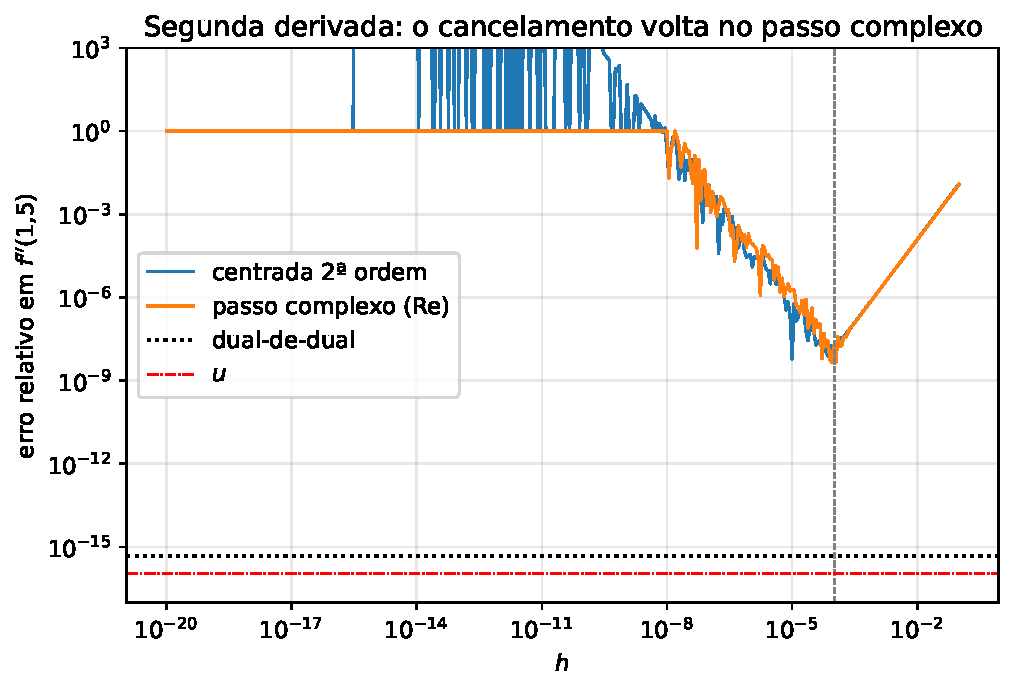
\includegraphics[width=0.75\textwidth]{figuras/a3_segunda_derivada.pdf}
\caption{Erro relativo de $f''(1{,}5)$. O passo complexo (parte real) tem o mesmo ``V'' da diferença centrada de segunda ordem. A linha pontilhada é o dual aninhado.}
\label{fig:a3}
\end{figure}

\paragraph{O que isso diz sobre os limites do truque.} O passo complexo funciona para $f'$ por uma razão estrutural: a parte imaginária \emph{começa} no termo de interesse, $hf'(x)$, sem nenhum termo $O(1)$ a ser removido. Para a parte real, o termo de interesse $h^2f''/2$ está atrás de $f(x)$, e removê-lo exige subtrair. Um único ``$\mathrm i$'' só isola uma derivada. Para derivadas de ordem superior sem cancelamento são necessárias várias unidades imaginárias independentes (números multicomplexos) ou, no lado da AD, duais aninhados/hiperduais: com $x = (x_0+\varepsilon_1)+(1+0\varepsilon_1)\varepsilon_2$, o coeficiente de $\varepsilon_1\varepsilon_2$ é $f''(x_0)$ exata. No notebook isso dá $f''(1{,}5)$ com erro relativo $4{,}9\times10^{-16}$, sem nenhum $h$.


%======================================================================
\begin{thebibliography}{9}
\bibitem{squire1998} W.~Squire e G.~Trapp. Using complex variables to estimate derivatives of real functions. \emph{SIAM Review}, 40(1):110--112, 1998.
\bibitem{martins2003} J.~R.~R.~A. Martins, P.~Sturdza e J.~J. Alonso. The complex-step derivative approximation. \emph{ACM Transactions on Mathematical Software}, 29(3):245--262, 2003.
\bibitem{baydin2018} A.~G. Baydin, B.~A. Pearlmutter, A.~A. Radul e J.~M. Siskind. Automatic differentiation in machine learning: a survey. \emph{Journal of Machine Learning Research}, 18(153):1--43, 2018.
\bibitem{griewank2008} A.~Griewank e A.~Walther. \emph{Evaluating Derivatives: Principles and Techniques of Algorithmic Differentiation}. 2.\,ed., SIAM, 2008.
\bibitem{higham2002} N.~J. Higham. \emph{Accuracy and Stability of Numerical Algorithms}. 2.\,ed., SIAM, 2002.
\end{thebibliography}

\end{document}
